\section{オートエンコーダ(Autoencoder)}
2006年にジェフリー・ヒントンらによって提案された\cite{autoencoder}オートエンコーダは,入力データを圧縮するエンコーダ(Encoder)部分と,圧縮されたデータを復元するDecoder(デコーダ)部分から構成されるニューラルネットワークである.\cite{unsupervised} \\
% オートエンコーダの構造を図\ref{fig:autoencoder}に示す.
一般的なオートエンコーダのエンコーダは,入力データの次元数を入力層のノード数とし,
中間層のノード数を層が深くなるほど入力データの次元数よりも小さくする.\\
デコーダは,エンコーダと次元数の構成が鏡になるように構成される.したがって,デコーダの入力次元数は,エンコーダの出力次元数であり,出力層は,エンコーダの入力の次元数と同じ次元数を持つ.\\
このような構造を持つオートエンコーダは,未完備オートエンコーダとも呼ばれ,
次元圧縮や,ノイズ除去などに用いられる.\\
また,逆にエンコーダの出力次元数を入力の次元数よりも大きくしたオートエンコーダは,
過完備オートエンコーダと呼ばれる.しかし,一般に呼称されるオートエンコーダとは,未完備オートエンコーダのことであり,過完備オートエンコーダとは役割や機能が全く異なることから,この先の説明では,オートエンコーダ=未完備オートエンコーダとして扱う.\\
本研究でも未完備オートエンコーダを用いて,実験・検証を行う.\\

オートエンコーダの学習は,入力データと出力データの誤差を最小化するように,中間層の重みを更新することで行われる.\\

オートエンコーダは学習において,中間層で圧縮され部分的に失われたデータから入力データ復元しようとするため,入力データの重要な特徴を抽出することが可能である.\\

% \begin{figure}[htbp]
%     \begin{center}
%         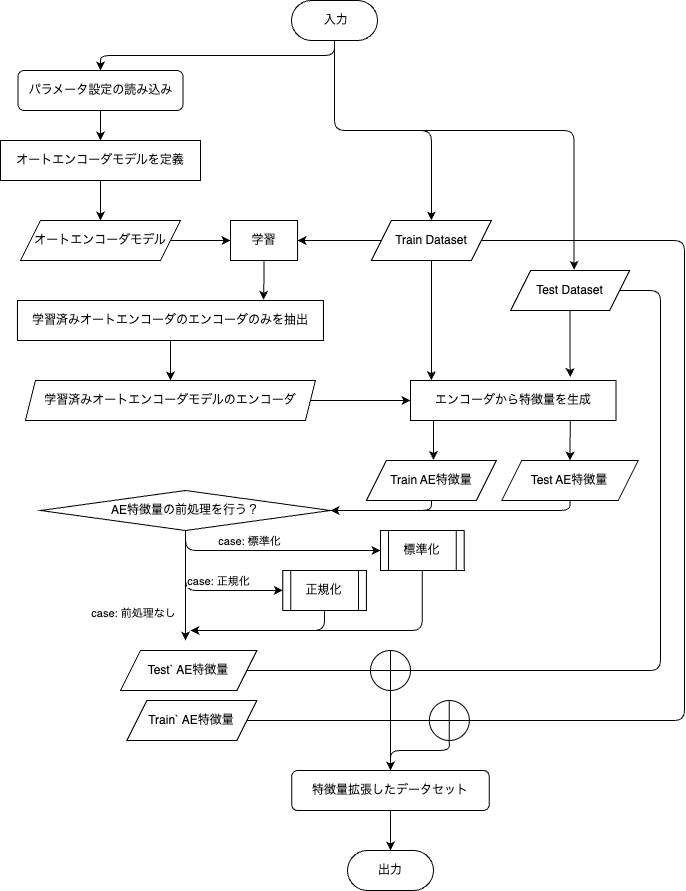
\includegraphics[width=10cm]{figures/autoencoder.png} % TODO: 
%         \caption{オートエンコーダの構造}
%         \label{fig:autoencoder}
%     \end{center}
% \end{figure}
